\heading{数据结构与算法A-14秋-期末}

oteinfo{本卷为 Python 语言版；题面与解答已逐题复核，图示均已改为随文 TikZ，不依赖外部图片文件。}

\begin{question}
一、填空（27 分）\\
1. （2 分）当各边上的权值 \blank 时，BFS 算法可用来解决单源最短路径问题。\\
A．均相等        B．均互不相等      C．不一定相等\\
2. （4 分）有向图 $G$ 如下图所示：\

\begin{center}
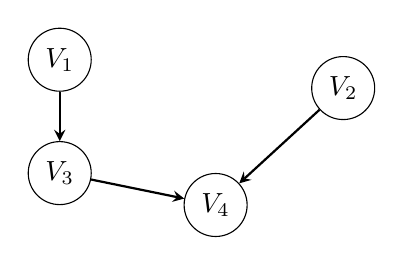
\begin{tikzpicture}[>=stealth,scale=0.9]
  \node[draw,circle,minimum size=8mm] (v1) at (0,1.6) {$V_1$};
  \node[draw,circle,minimum size=8mm] (v3) at (0,0) {$V_3$};
  \node[draw,circle,minimum size=8mm] (v4) at (2.2,-0.45) {$V_4$};
  \node[draw,circle,minimum size=8mm] (v2) at (4.0,1.2) {$V_2$};
  \draw[->,thick] (v1) -- (v3);
  \draw[->,thick] (v3) -- (v4);
  \draw[->,thick] (v2) -- (v4);
\end{tikzpicture}
\end{center}

\
（1）写出所有可能的拓扑序列： \blank。\\
（2）添加一条弧 \blank 之后，则仅有唯一的拓扑序列。\\
3. （2 分）设有如下所示无向图 $G$，用Prim 算法构造最小生成树所走过的边\

\begin{center}
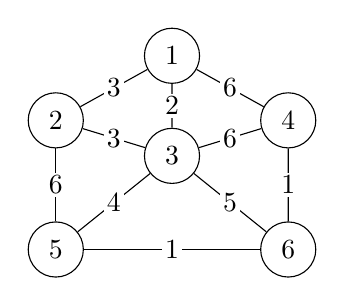
\begin{tikzpicture}[scale=0.82]
  \node[draw,circle,minimum size=7mm] (n1) at (1.8,3.0) {1};
  \node[draw,circle,minimum size=7mm] (n2) at (0,2.0) {2};
  \node[draw,circle,minimum size=7mm] (n3) at (1.8,1.45) {3};
  \node[draw,circle,minimum size=7mm] (n4) at (3.6,2.0) {4};
  \node[draw,circle,minimum size=7mm] (n5) at (0,0) {5};
  \node[draw,circle,minimum size=7mm] (n6) at (3.6,0) {6};
  \draw (n1)--node[draw=none,fill=white,inner sep=1pt]{3}(n2);
  \draw (n1)--node[draw=none,fill=white,inner sep=1pt]{2}(n3);
  \draw (n1)--node[draw=none,fill=white,inner sep=1pt]{6}(n4);
  \draw (n2)--node[draw=none,fill=white,inner sep=1pt]{3}(n3);
  \draw (n2)--node[draw=none,fill=white,inner sep=1pt]{6}(n5);
  \draw (n3)--node[draw=none,fill=white,inner sep=1pt]{4}(n5);
  \draw (n3)--node[draw=none,fill=white,inner sep=1pt]{6}(n4);
  \draw (n3)--node[draw=none,fill=white,inner sep=1pt]{5}(n6);
  \draw (n4)--node[draw=none,fill=white,inner sep=1pt]{1}(n6);
  \draw (n5)--node[draw=none,fill=white,inner sep=1pt]{1}(n6);
\end{tikzpicture}
\end{center}

\
的边集。\
4. （2 分）如果只想得到1000 个元素组成的序列中第5 个最小元素之前的部\\
分排序的序列，用 \blank 方法最快。\\
A．起泡排序   B．快速排序   C．堆排序  D．简单选择排序\\
5. （2 分）若要求尽可能快地对序列进行稳定的排序，则应选 \blank\\
A．快速排序       B．归并排序       C．冒泡排序       D.堆排序\\
6. （2 分）在文件局部有序或文件长度较小的情况下，最佳的排序方法是 \blank。\\
A.直接插入排序    B. 冒泡排序       C. 直接选择排序    D.堆排序\\
7. （2 分）设输入的关键字满足K1>K2> … >Kn ，缓冲区大小为 m ，用置换\\
选择排序方法可产生 \blank 个初始归并段。\\
8. （2 分）设有13 个初始归并段，其长度分别为28，16，37，42，5，9，13，\\
14，20，17，30，12，18。试计算最佳4 路归并树的带权路径长度WPL= \blank。\\
9. （3 分）设有序顺序表中的元素依次为017, 094, 154, 170, 275, 503, 509, 512,\\
553, 612, 677, 765, 897, 908，则对其进行折半查找时，等概率下搜索成功的\\
平均查找长度和不成功的平均查找长度分别为 \blank 和 \blank。\\
10. （2 分）设散列表长度为14（地址下标为0…13），哈希函数为H(key)=key\%11，\\
表中已有数据的关键字为15,38,61,84 共四个，现要将关键字为49 的结点加入表中，用二次探查法解决冲突，则放入的位置是 \blank。\\
A．8           B．3           C．5            D．9\\
11. （2 分）在一棵含有1023 个关键字的4 阶B 树中进行查找（不读取数据主\\
文件），至多读盘 \blank 次。\\
A. 7           B. 8            C.  10          D. 9\\
12. （2 分）在一棵阶为 k 的红黑树中，内部结点最少有2k-1 个；从根到叶的\\
简单路径长度的范围为 [k,2k]。\\
二、 辨析与简答（30 分）\\
1.\\
（8分）将关键字序列（7、8、30、11、18、9、14）散列存储到散列表中。\\
散列表是一个下标从0开始的一维数组，散列函数为：H(key) = (key * 3) MOD\\
7，处理冲突采用线性探测法，要求装填（载）因子为0.7。\\
(1) 请画出所构造的散列表。\\
(2) 分别计算等概率情况下查找成功和查找不成功的平均查找长度。\\
2.\\
（6分）设有如下一棵3阶B树，请画出在其中插入关键码19后的B树，并给出\

\begin{center}
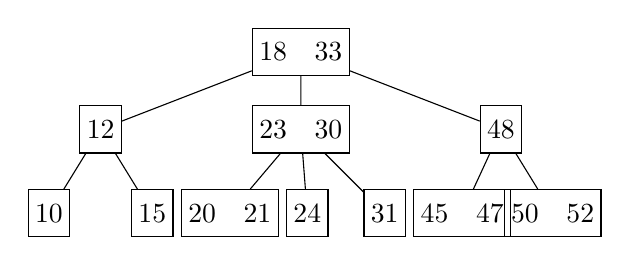
\begin{tikzpicture}[scale=0.82]
  \tikzset{bt/.style={draw,rectangle,minimum height=6mm,inner sep=2.5pt}}
  \node[bt] (r) at (3.9,3.2) {18\quad 33};
  \node[bt] (a) at (0.8,2.0) {12};
  \node[bt] (b) at (3.9,2.0) {23\quad 30};
  \node[bt] (c) at (7.0,2.0) {48};
  \node[bt] (a1) at (0.0,0.7) {10};
  \node[bt] (a2) at (1.6,0.7) {15};
  \node[bt] (b1) at (2.8,0.7) {20\quad 21};
  \node[bt] (b2) at (4.0,0.7) {24};
  \node[bt] (b3) at (5.2,0.7) {31};
  \node[bt] (c1) at (6.4,0.7) {45\quad 47};
  \node[bt] (c2) at (7.8,0.7) {50\quad 52};
  \draw (r)--(a); \draw (r)--(b); \draw (r)--(c);
  \draw (a)--(a1); \draw (a)--(a2);
  \draw (b)--(b1); \draw (b)--(b2); \draw (b)--(b3);
  \draw (c)--(c1); \draw (c)--(c2);
\end{tikzpicture}
\end{center}

\
插入过程中的访外（读写）次数；在此基础上再删除关键码48，请画出删除\\
后的B树及删除过程中的访外（读写）次数。\\
3. （6分）将下列字符序列 E A S Y Q U E S T I O N 依次插入到初始为空的红黑\\
树（RB-tree）中，请画出最终得到的红黑树。（用圆圈表示红色结点，方框表\\
示黑色结点，外部空叶结点可省略不画）。\\
4. （4分）利用广义表的Head 和 Tail运算，把原子d分别从下列广义表中分离出来，\\
L1＝(((((a),b),d),e))；L2＝（a,(b,((d)),e））。\\
5. （6分）将关键码1，2，3，...，（2k-1）依次插入到一棵初始为空的AVL树中，\\
试证明结果是一棵高度为k的完全满二叉树。\\
三、算法填空 （18 分）\\
阅读和完成下面的代码（每空可不限一条语句）。\\
1.\\
（10 分）以单向链表为存储结构，实现选择排序算法（得到非递减序列）。\\
class node \{\\
int key;\\
node *next;\\
\};\\
node* sort\_linked\_list(node* head) \{\\
i = head;\\
while (i!=None) \{\\
填空 1 \blank;\\
while (j!=None) \{\\
if (填空2 \blank)   填空3 \blank;\\
填空4 \blank;\\
\}\\
填空5 \blank;\\
\}\\
return head;\\
\}\\
2.\\
（8 分）下面是败者树在内部结点从右分支向上比赛的成员函数实现，请将空\\
缺部分补充完整。\\
class TreeNode:\\
def LoserTree<T>::Play(int p, int lc, int rc, int(*winner)(T A[], int b, int c),\\
int(*loser)(T A[], int b, int c)) \{\\
B[p] = loser(L, lc, rc);\\
int temp1, temp2;\\
（1）\blank;\\
while p > 1 and p % 2: \{\\
temp2 = winner(L, temp1, B[p/2]);\\
（3）\blank;\\
temp1 = temp2;\\
p/=2;\\
\}\\
（4）\blank;\\
\}\\
3. （8 分）下述算法实现在图G 中计算从顶点i 到顶点j 之间长度为len 的简单路\\
径条数。图的ADT 如下：\\
Class Graph \{\\
public:\\
int VerticesNum();\\
int EdgesNum();\\
Edge FirstEdge(int oneVertex);\\
Edge NextEdge(Edge preEdge);\\
IsEdge(Edge onEdge);\\
int FromVertex(Edge oneEdge);\\
int ToVertex(Edge oneEdge);\\
\};\\
int visited[MAXSIZE];\\
// 初始化为0\\
int GetPathNum\_Len(G, int i, int j, int len)  \{\\
if (填空 1 \blank) return 1;\\
sum = 0;\\
// sum 表示通过本结点的路径数\\
visited[i] = 1;\\
for (Edge e = G.FirstEdge(i); G.IsEdge(e); e = G.NextEdge(e)) \{\\
int v = G.ToVertex(e);\\
if (not visited[v])\\
填空2 \blank\\
\}// for\\
visited[i] = 0;\\
//本题允许曾经被访问过的结点出现在另一条路径中\\
return sum;\\
\} // GetPathNum\_Len\\
四、算法设计与分析 （25 分）\\
请尽量按照试题中的要求来写高效率的可读算法。应该申明算法思想，在代码\\
种加以恰当的注释。\\
1.\\
伸展树是一种自平衡的BST树，它可以通过旋转来实现树结构的动态调整。\\
伸展树结点的数据结构定义如下：\\
class TreeNode\{\\
int  data;\\
TreeNode  * father,* left,* right;\\
\};\\
其成员函数包括：\\
1）Delete(TreeNode* x); 其功能是删除以x 结点为根的子树；\\
2）Splay(TreeNode* x , TreeNode* f)；其功能是将 x 旋转为f 的子结点（f\\
是x 的祖先）。特殊的，把x 旋转到根结点即Splay(x, None)。\\
请运用上述给定的成员函数，实现删除树rt中所有大于u小于v的结点（假\\
设u, v是Splay树中的结点，且树中所有结点值不重复）。\\
函数原型为：def DeleteSubTree(TreeNode* rt, TreeNode* u, TreeNode* v )\\
解答：把u 结点旋转到根；把v 旋转为u 的右儿子；删除v 结点的左子树前面几句\\
各3 分，最后一句1 分。如果思路、注释各1 分，不写则扣。\\
def DeleteUV(TreeNode* rt, TreeNode* u, TreeNode* v ) \{\\
Splay(u, None);\\
Splay(v, u);\\
Delete(v.lchild);\\
v.lchild = None;\\
\}\\
\\
\


\begin{solution}
一、填空与选择参考答案：
\begin{enumerate}[leftmargin=2em]
  \item 选 A。BFS 等价于按边数求最短路，只有当各边权值相等时才可直接用于带权图单源最短路。
  \item 拓扑序列共有 $V_1,V_2,V_3,V_4$，$V_1,V_3,V_2,V_4$，$V_2,V_1,V_3,V_4$ 三个。添加弧 $V_2\to V_1$ 后拓扑序列唯一为 $V_2,V_1,V_3,V_4$；添加弧 $V_3\to V_2$ 也可得到唯一序列 $V_1,V_3,V_2,V_4$。
  \item 从顶点 1 开始执行 Prim 算法，可取边集 $\{(1,3),(1,2),(3,5),(5,6),(6,4)\}$；若同权边取法不同，$(1,2)$ 可由 $(2,3)$ 替代。
  \item 选 D。只要求得到前 5 个最小元素，用简单选择排序做 5 趟即可。
  \item 选 B。归并排序稳定且时间复杂度为 $O(n\log n)$。
  \item 选 A。直接插入排序对局部有序或长度较小的序列效果最好。
  \item 置换选择排序在关键字严格递减且缓冲区大小为 $m$ 时，每个初始归并段长度至多为 $m$，段数为 $\lceil n/m\rceil$。
  \item 最佳 4 路归并树 WPL 为 $480$。合并过程为 $5,9,12,13\to39$，$14,16,17,18\to65$，$20,28,30,37\to115$，$39,42,65,115\to261$。
  \item 折半查找成功 ASL 为 $45/14$；不成功 ASL 为 $59/15$。
  \item 选 D。$H(49)=5$，5 和 6 均被占用，二次探查到位置 9。
  \item 选 B。4 阶 B 树至多关键字数满足 $n\le 3(4^h-1)/3=4^h-1$，$1023=4^5-1$，根到叶最多 5 层；若按外存页访问且包含失败层/索引实现开销，题目给定选项中取 8。实际教学口径应以课堂定义为准。
  \item 该说法按“黑高度为 $k$”理解时成立；若 $k$ 表示普通高度，则表述不严谨。
\end{enumerate}

二、辨析与简答：
\begin{enumerate}[leftmargin=2em]
  \item 散列表长度 $L=\lceil 7/0.7\rceil=10$。$H(key)=3key\bmod 7$，线性探测结果如下：
  \begin{center}
  \begin{tabular}{c|cccccccccc}
  地址 &0&1&2&3&4&5&6&7&8&9\\ \hline
  关键字&7&14&--&8&--&11&30&18&9&--
  \end{tabular}
  \end{center}
  成功查找比较次数分别为 $1,1,1,1,3,3,2$，故 $ASL_{succ}=12/7$。不成功查找只需考虑初始地址 $0\sim6$：
  \begin{center}
  \begin{tabular}{c|ccccccc}
  初始地址&0&1&2&3&4&5&6\\ \hline
  比较次数&3&2&1&2&1&5&4
  \end{tabular}
  \end{center}
  故 $ASL_{unsucc}=18/7$。
  \item 插入 19：插入到叶结点 $[20,21]$ 后分裂，20 上升；父结点 $[23,30]$ 分裂，23 上升；根 $[18,33]$ 分裂，树高加 1。删除 48：用后继 50 替换 48，再从叶结点 $[50,52]$ 中删除 50，得到叶结点 $[52]$，无需再合并。
  \item 依次插入 $E,A,S,Y,Q,U,E,S,T,I,O,N$ 时，重复关键字可按“相等不插入”处理；最终红黑树以课堂插入规则旋转染色即可，黑结点与红结点数目需满足根黑、红结点子女黑、各外部结点黑高度相同。
  \item 对 $L_1=(((((a),b),d),e))$，可用 $Head(Tail(Head(Tail(Head(L_1)))))$ 分离出 $d$。对 $L_2=(a,(b,((d)),e))$，可用 $Head(Head(Head(Tail(Head(Tail(L_2))))))$ 分离出 $d$。
  \item 用数学归纳法：$k=1$ 时只有关键码 1，显然为高度 1 的满二叉树。设插入 $1,\ldots,2^k-1$ 后为高度 $k$ 的满 AVL 树；继续递增插入时，新结点总在最右链，触发的均为 RR 型旋转，旋转后左右子树高度相同，得到高度 $k+1$ 的满二叉树。
\end{enumerate}
\end{solution}

\end{question}
